\documentclass{article}

\usepackage[a4paper]{geometry} % document dimensions
\usepackage{amsmath} % multiline equation numbering
\usepackage{amssymb} % e.g. triangleq, checkmark
\usepackage{textcomp,gensymb} % \degree symbol
\usepackage[T1]{fontenc} % support accents via UTF

\usepackage{graphicx} % support for graphics
\usepackage[hidelinks]{hyperref} % hyperlinks and autoref
\hypersetup{
    pdfauthor={Nick Ackerley, Graeme Weatherill},
    pdfsubject={Engineering Seismology},
    pdftitle={Method of collapsing epistemic uncertainty in frequency-magnitude distributions for regional seismic hazard models},
    pdfkeywords={seismology, hazard, India, OpenQuake}}
\usepackage{natbib} % bibliography support
\usepackage{adjustbox} % support for too-wide figures
\usepackage{caption} % support for captions of floats
\providecommand*\hyphen{-} % dashed page numbers in bib

\usepackage{enumitem} % control list formatting
\setlist{noitemsep}

%%% PREAMBLE

% numeric "thanks" footnotes
\makeatletter
\let\@fnsymbol\@arabic
\makeatother

\begin{document}

\title{Method of collapsing epistemic uncertainty in frequency-magnitude distributions for regional seismic hazard models}
\date{December 31, 2016}

\author{
Nick Ackerley
\thanks{Istituto Universitario di Studi Superiori, Pavia, Italy} \textsuperscript{,}
\thanks{Geological Survey of Canada, Ottawa, Canada} \and 
Graeme Weatherill
\thanks{Global Earthquake Model (GEM), Pavia, Italy} }

\maketitle
\begin{abstract}
Logic trees are an accepted way of modelling epistemic uncertainty in seismic hazard. 
Source model logic trees pose no particular computational difficulty in site-specific studies involving on the the order of ten source zones and a small number of sites. 
Regional or national hazard models can require on the order of a hundred zones, however, and in these cases, with a relatively simple source model logic tree with on the order of ten branches, the hazard integral can turn out to be too computationally intensive to compute. 

We show that in a classical probabilistic seismic hazard assessment, the complexity of a mean hazard calculation can be drastically reduced by ``collapsing'' the epistemic uncertainty for each source zone, prior to computation of the hazard integral. 
Our result is exact but is available only for the mean hazard. 
Full enumeration of logic trees is still required to obtain an exact result for medians or other quantiles, however we propose procedures for pruning of trees which can greatly reduce the complexity of such computations while introducing negligible error. 
\end{abstract}

\section{Introduction}

The established procedure for incorporating epistemic uncertainties in probabilistic seismic hazard models is to construct logic trees to weight different possible models \citep{bommer2008use}. 
Ground-motion prediction equations (GMPEs), for example, are assigned weights according to the likelihood that each is representative for a given source zone \citep{delavaud2012toward, ceus2012central}. 
It is routine to further weight different models of seismicity \citep{ field2014uniform, woessner2015european}, specifically frequency-magnitude distributions (FMDs), which could give rise to the actual instrumental, historic and paleoseismic records. 
Assignment of logic tree weights to maximum magnitude is common, but different b-values are also sometimes weighted independently.
When applying these methods to a site-specific study, no particular difficulty arises.

Regional models can have hundreds of source zones, each with its own logic trees for GMPEs and FMDs.
For full enumeration of the logic tree for such a model the number of source zones must be raised to the power of the total number of logic tree branches.
Because of this, methods for the reduction of logic tree branches are crucial.
Procedures for assessing the appropriateness of GMPEs include data-driven \citep{scherbaum2009model, kale2013new} and non-data-driven \citep{bommer2010selection} approaches.
This means there are numerous strategies for reducing GMPE logic trees to the minimum necessary complexity.
Aside from noting that it is inappropriate to treat a- and b-values as independent variables in FMD logic trees \citep{bommer2008use}, little guidance exists for the reduction of FMD logic tree complexity.
Partial enumeration of the logic tree is one means to reduce computational complexity, but it is not clear how one can ensure that the subset chosen properly represents the spread of the distribution.

In the next section it is shown that the mean hazard can be computed exactly by ``collapsing'' the FMDs prior to evaluation of the hazard integral.
A simple case study for which the mean hazard can be computed by full enumeration follows. 
It is shown that the mean hazard is exact as long as the mean annual rate of exceedance is sufficiently low. These results are discussed and their ramifications for regional seismic hazard models are explored.
Finally, methods for pruning logic trees of complex regional models are discussed.

\section{Computation of mean hazard given epistemic uncertainty}

In classical PSHA the hazard integral gives an estimate of rate at which the ground motion $Y$ at a site of interest will exceed some value $y$. 
For a set of $N_S$ sources generating ruptures of $N_M$ magnitudes $m_j$ at $N_R$ distances $r_k$ using discrete summations,  \citep{baker2008introduction}:

\begin{equation} \label{eq:HazardIntegral} 
\lambda(Y > y) = 
\sum_{i=1}^{N_S} 
\lambda(M_i > m_\text{min}) 
\sum_{j=1}^{N_M} 
\sum_{k=1}^{N_R} 
P_i(Y > y|m_j,r_k) 
P_i(M_i=m_j) 
P_i(R_i=r_k)
\end{equation}

Where for source $i$:
\begin{itemize}
\item $\lambda_i(M_i > m_\text{min})$ is the rate of earthquakes greater than $m_\text{min}$
\item $P_i(Y > y|m_j,r_k)$ is the ground motion prediction equation (GMPE) and incorporates aleatory uncertainty in the ground motion
\item $P_i(M_i=m_j)$ is the frequency-magnitude distribution (FMD)
\item $P_i(R_i=r_k)$ is the distribution of distance measures from points within the source to the site of interest.
\end{itemize}

For a single point source, neglecting finite source effects, this simplifies to:

$$ \lambda(Y > y) = 
\lambda(M > m_\text{min}) 
\sum_{j=1}^{N_M} 
P(Y > y|m_j,R) 
P(M=m_j) $$

But now suppose that certain epistemic uncertainties have been identified. 
In order to estimate the effect of this lack of knowledge on the mean and spread of ground motions suppose $N_G$ GMPEs $P_\ell(Y > y|m_j,R)$ have been assigned weights $w_\ell$ and $N_F$ FMDs $P_m(M=m_j)$ have been assigned weights $w_m$. 
Now

$$ \lambda(Y > y) = 
\lambda(M > m_\text{min}) 
\sum_{m=1}^{N_F} w_m 
\sum_{\ell=1}^{N_G} w_\ell 
\sum_{j=1}^{N_M} 
P_\ell(Y > y|m_j,R) 
P_m(M=m_j) $$

Since we can reorder the summations to obtain

$$ \lambda(Y > y) = 
\lambda(M > m_\text{min}) 
\sum_{\ell=1}^{N_G} w_\ell 
\sum_{j=1}^{N_M} 
P_\ell(Y > y|m_j,R) 
\sum_{m=1}^{N_F} w_m 
P_m(M=m_j) $$

We can pre-compute the ``collapsed'' FMD for the source:

$$ P_C(M=m) \equiv \sum_{m=1}^{N_F} w_m P_m(M=m) $$

And this simplifies the hazard summation to

$$ \lambda(Y > y) = 
\lambda(M > m_\text{min}) 
\sum_{\ell=1}^{N_G} w_\ell 
\sum_{j=1}^{N_M} 
P_\ell(Y > y|m_j,R) 
P_C(M=m_j) $$

Note that a similar ``collapse'' of GMPE uncertainty is not possible because the ground motion is conditional upon the magnitude. [check again and clarify!]

Returning to the case of multiple sources, we can include ground-motion and frequency-magnitude epistemic uncertainty by writing:

$$ \lambda(Y > y) = 
\sum_{i=1}^{N_S} 
\lambda_i(M_i > m_\text{min}) 
\sum_{m=1}^{N_F} w_{m,i} 
\sum_{\ell=1}^{N_G} w_{\ell,i}
\sum_{j=1}^{N_M} 
\sum_{k=1}^{N_R} 
P_{\ell,i}(Y > y|m_j,r_k) 
P_{m,i}(M_i=m_j) 
P_i(R_i=r_k) $$

We can still reorder the summations, as long as we recognize that the collapsed FMD is different for each source

$$
\lambda(Y > y) = 
\sum_{i=1}^{N_S} 
\lambda(M_i > m_\text{min}) 
\sum_{\ell=1}^{N_G} w_{\ell,i}
\sum_{j=1}^{N_M} 
\sum_{k=1}^{N_R} 
P_{\ell,i}(Y > y|m_j,r_k) 
P_i(R_i=r_k) 
\sum_{m=1}^{N_F} w_{m,i} 
P_{m,i}(M_i=m_j) 
$$

So that for source $i$ the collapsed FMD is

\begin{equation} \label{eq:CollapsedFmd} 
P_{Ci}(M_i = m) \equiv
\sum_{m=1}^{N_F} w_{m,i} 
P_{m,i}(M_i=m) 
\end{equation}

The important point here is that the ``collapsed'' FMD can be pre-computed for each source. 
The number of logic tree branches in full enumeration after collapsing FMD uncertainty, and thus the computation complexity and time, are thus greatly reduced.

\section{Case Study: Guwahati}

The effectiveness of this method of ``collapsing'' FMD logic trees is demonstrated using a case study for the city of Guwahati in India.
The source regions, GMPE and FMD logic trees used are part of an implementation \citep{ackerley2017open} using the OpenQuake platform \citep{pagani2014openquake} of a PSHA model for the Indian subcontinent \citep{nath2012probabilistic}. 
\autoref{fig:CollapsedFmd} shows an example of the pre-computation of collapsed FMDs as described in equation \eqref{eq:CollapsedFmd} for a single zone.

\begin{figure}[!htb]
\begin{adjustbox}{center}
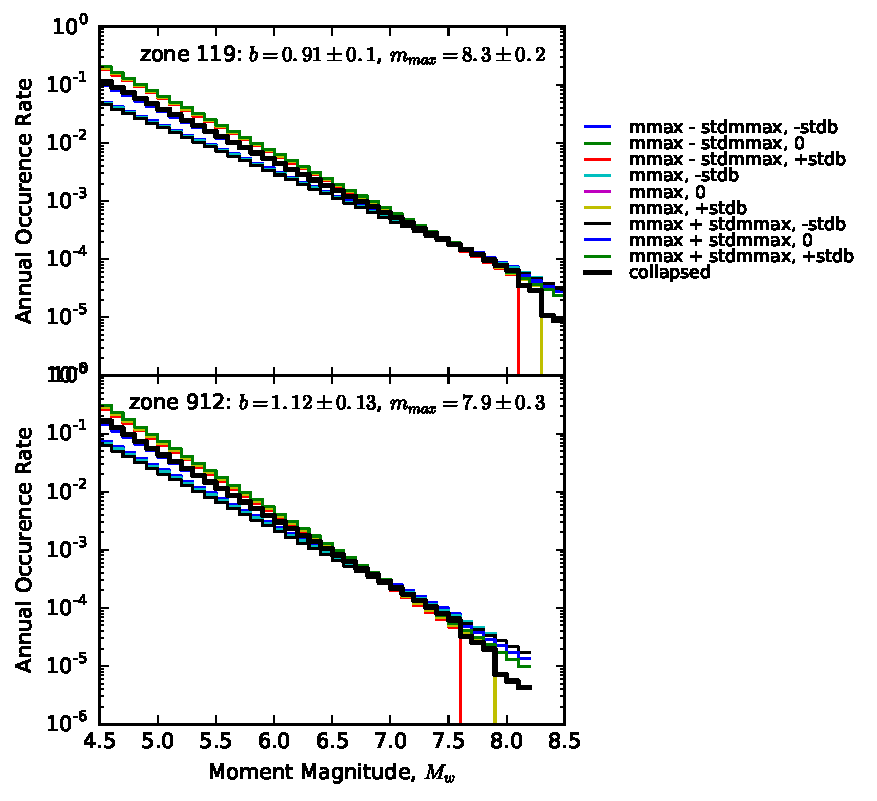
\includegraphics{Mean_Occurrence_Rates_Zones_119_912}
\end{adjustbox}
\caption[Frequency-magnitude distributions for two zones nearest to Guwahati, India]{Frequency-magnitude distributions corresponding to various branches of the logic tree of \cite{nath2012probabilistic}. 
The zones chosen are the two closest to Guwahati, India. 
Zone 119 at 25-50 km depth is the zone capable of producing a devastating ``pop-up'' type event \citep{Bilham2001, nath2012ground}. 
The ``collapsed'' FMD uncertainty computed using \eqref{eq:CollapsedFmd} is shown as a heavy black line.} 
\label{fig:CollapsedFmd}
\end{figure}

In order to show the effectiveness of ``collapsing'' FMD logic trees a greatly simplified subset of the full regional model was used.
In particular, a single site (Guwahati), and just two areal source zones (one with the FMD shown in \autoref{fig:CollapsedFmd} plus another zone the same FMD logic tree structure) were considered.
This makes it possible to rapidly compute the hazard by fully enumerating the logic trees.

With this extremely simplified model the computation time dropped by a factor of 40 when FMD uncertainty was collapsed. 
In realistic regional models, with gridded sites and hundreds of areal sources, each with FMD uncertainty, the computational savings are far greater, and can make an intractable problem tractable. 

The analysis of the previous section predicts that collapsed FMDs should give an exact result for the mean exceedance rate. 
\autoref{fig:MeanFullVsCollapsed} in fact shows that this procedure gives a very good approximation of the mean hazard for low but not for high probabilities of exceedance. 

[Some further investigation is needed to find out what determines this threshold; if it is dependent on the return period chosen alone then inaccuracy at low-probability of exceedance is effectively a computational artefact, a curiosity of no engineering significance. 
Another possibility is that it is a result of the discretisation of the FMD used; in this case it would be possible to reduce the error by discretise the FMDs using bin widths of say 0.01 magnitude units instead of 0.1, but there would be a corresponding computational penalty.

Perhaps it would be better to attempt a theoretical treatment of the errors. Conceivably it is the fully-enumerated model which is in error! A reference as a starting point would be good.]

\begin{figure}[!htb]
\begin{adjustbox}{center}
\includegraphics{Guwahati_mean_Zones_119_912_1year.pdf}
\end{adjustbox}
\caption[Mean hazard curves computed using various levels of FMD uncertainty]{Mean hazard curves computed using various levels of FMD uncertainty. 
The site of interest is the city of Guwahati. 
The source model consists only of zones 119 and 912 of \cite{nath2012probabilistic}. 
The full GMPE logic tree of \cite{nath2012probabilistic} is used. 
The ``fully enumerated'' result implements the FMD logic tree described in \cite{nath2012probabilistic} while ``collapsed'' implements \eqref{eq:CollapsedFmd} and ``no FMD uncertainty'' models only the FMD logic tree branches with the largest weights.} 
\label{fig:MeanFullVsCollapsed}
\end{figure}

Unfortunately the ``collapse'' of logic trees in source zones is of no use in computing the median or any other quantile of hazard.
\autoref{fig:MedianFullVsCollapsed} demonstrates, for the same simplistic example, that the error in the calculated median hazard is much too large, as large as if epistemic uncertainty in source seismicity was neglected entirely.
The problem is that the most basic procedure for calculating a quantile is to compute the hazard for all (every combination of all branches of all) realizations of the logic trees and then sort them.
The hazard at a given quantile is unaffected by the values of hazard at other quantiles except inasmuch as it might affect sort order near the specified quantile.

\begin{figure}[!htb]
\begin{adjustbox}{center}
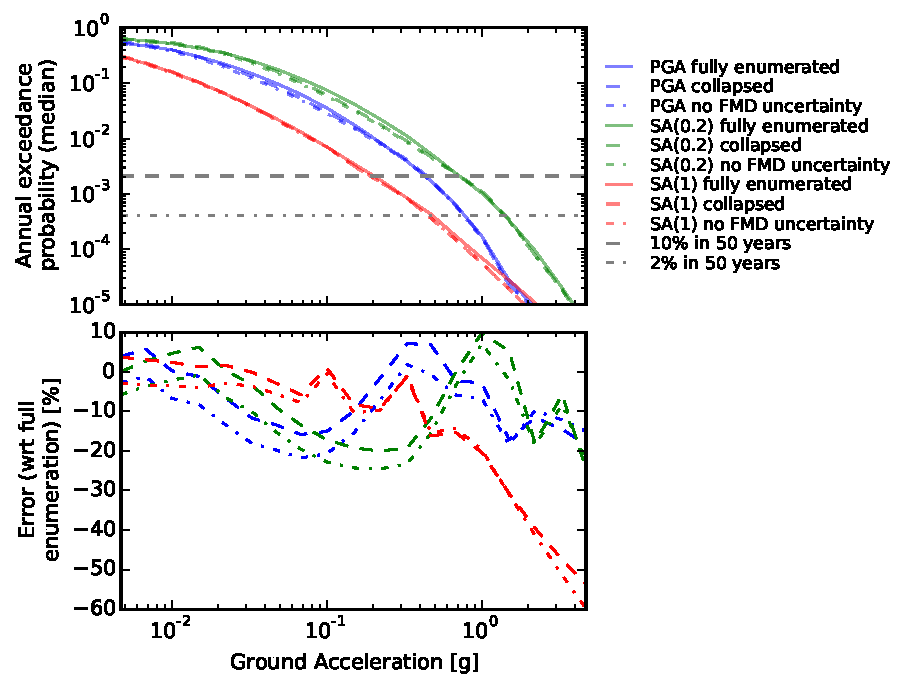
\includegraphics{Guwahati_median_Zones_119_912_1year}
\end{adjustbox}
\caption[Median hazard curves computed using various levels of FMD uncertainty]{Median hazard curves computed using various levels of FMD uncertainty. 
For detailed description see \autoref{fig:MeanFullVsCollapsed}} 
\label{fig:MedianFullVsCollapsed}
\end{figure}

\section{Discussion}

The ``collapse'' of FMD logic trees is practicable in using any software package capable of implementing arbitrary FMDs.
However this method's utility would be much greater if it were implemented directly in the software.
Seismic hazard models are typically specified as an interrelated set of files describing geometry and other characteristics of the source zones, GMPE logic trees and FMD logic trees.
If the user has to recompute the source zone characteristics in order to eliminate the FMD logic trees and calculate mean hazard, then one effectively cannot use that same model to compute the median hazard.
If on the other hand the software can be relied upon to take the full FMD logic trees as input and ''collapse`` them when appropriate (i.e. when only the mean hazard is requested), then the same model can then be used to be compute medians and other quantiles. 
This is an important benefit, because mean hazard is an important indicator of quality assurance, and the ability to compute it quickly permits more rapid development of complex models as the regional scale and beyond.

Finally a few words about possible efficiencies in the computation of hazard quantiles.
Aleatory variability is modelled in most if not all GMPEs using a log-normal distribution so the ability to compute an arbitrary quantile of ground-motion exceedance is built-in. 
For epistemic variability the first step in evaluating quantiles is simply the enumeration of the possible realizations, but even this can pose a problem for regional models.
For a region with $N_S = 64$ sources, each with $N_B = 8$ frequency-magnitude distribution logic-tree branches and $N_G = 4$ GMPE logic-tree branches the total number of logic tree realizations would be $N = (N_B N_G)^{N_S} = (2^5)^{2^6} = 2^{320}$. 
This is much larger than the largest integer representable on a 64-bit computer and thus the realizations are thus effectively uncountable without extra precautions.
Fortunately, depending on the expected level of hazard in a sub-region, and the relative levels of seismicity in nearby sources, it is generally possible to set a cutoff radius (e.g. 200 km), beyond which source zones need not be considered.
For the same regional model with 64 sources, suppose only $N_S'= 8$ source zones are within the cutoff radius. 
Suddenly the total number of logic tree realizations is reduced to $N' = (N_B N_G)^{N_S^\prime} = (2^5)^{2^3} = 2^{40}$, a much more manageable number.
Effectively most of the logic tree branches can be ``pruned'' away by this process.
It should furthermore be possible to come up with an efficient procedure to find subsets of gridded sites within a region which have the same set of source zones within the cutoff radius, allowing significant reuse of subsets of the hazard calculation.
Implementation of logic tree pruning in a hazard calculation platform such as OpenQuake would enable the calculation of hazard quantiles for regional models.

\section{Conclusions}

The ``collapse'' of FMD logic trees by weighted summation of branches yields identical results to full enumeration as long as the annual probability of exceedance is low.


\bibliographystyle{apalike}
\bibliography{/home/nick/Desktop/Library/PSHA.bib,/home/nick/Desktop/Library/india-hazard.bib}

\end{document}